%%%%%%%%%%%%%%%%%%%%%%%%%%%%%%%%%
%
%       EXERCÍCIO
%
%%%%%%%%%%%%%%%%%%%%%%%%%%%%%%%%%

\ifdefstring{\atividade}{prova}{%
    \ifdefstring{\modo}{objetivo}{%
        \renewcommand{\valorquestao}{\ValorQObj\ ponto}
    }{%
        \renewcommand{\valorquestao}{\ValorQDisc\ pontos}
    }%
}%

\begin{exercicioBanco}[\valorquestao]
Considere a função afim cujo gráfico está desenhado abaixo.
%

%
\begin{center}
    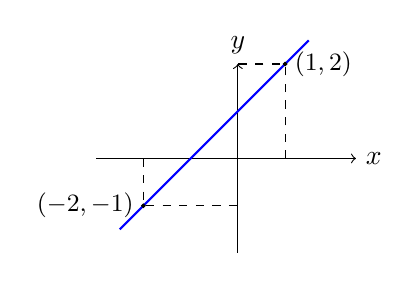
\begin{tikzpicture}[scale=0.6]
        % Eixos
        \draw[->] (-3,0) -- (2.5,0) node[right] {\(x\)};
        \draw[->] (0,-2) -- (0,2) node[above] {\(y\)};
              
        % Gráfico
        \draw[domain=-2.5:1.5, smooth, variable=\x, blue, thick] 
        plot ({\x}, {\x+1});
              
        % Pontos escolhidos
        \draw[dashed] (-2,0) -- (-2,-1) -- (0,-1);
        \draw[dashed] (1,0) -- (1,2) -- (0,2);
             
        % Marcando os pontos
        \filldraw (-2,-1) circle (1pt) node[left] {\small\((-2,-1)\)};
        \filldraw (1,2) circle (1pt) node[right] {\small\((1,2)\)};
    \end{tikzpicture}
\end{center}
%
Determine o zero dessa função.

% Define as alternativas
\newcommand{\alternativas}{%
    \begin{center}
        \begin{tabularx}{\textwidth}{XXXXX}
            (a) \(-2\). &
            (b) \(-1\). &
            (c) \(0\). &
            (d) \(1\). &
            (e) \(2\).
        \end{tabularx}
    \end{center}
}

% Define a resposta correta
\newcommand{\resposta}{B}

% Lógica condicional para exibição
\ifdefstring{\atividade}{lista}{%
    \alternativas
    \vspace{0.5em}
    
    \noindent\textbf{Resposta:} letra \textbf{\resposta}.
}{%
    \ifdefstring{\modo}{objetivo}{%
        \alternativas
    }{%
        % modo = discursiva → não mostra alternativas
    }
}
\end{exercicioBanco}

